\section{Деревья поиска}
Корневое дерево:
бинарное дерево,
дерево с произвольным ветвлением,
представление <<левый ребёнок --- правый сосед>>.
Дерево поиска: поиск, вставка, удаление,
поиск следующего и предыдущего элемента за время,
пропорциональное высоте.
АВЛ-дерево: верхняя оценка $\O(\log n)$ на высоту,
сохранение свойства при помощи малых и больших вращений.

\subsection{Дерево поиска}
Корневое дерево --- дерево с выделенным корнем.
Бинарное дерево --- у каждой вершины не более 2 детей.
Любое дерево можно представить в виде бинарного,
в представлении <<левый ребёнок --- правый сосед>>:

\begin{center}
    \begin{tikzpicture}
        \node at (0, 0) (x1) {1};
        \node at (-1, -1) (x2) {2};
        \node at (0, -1) (x3) {3};
        \node at (1, -1) (x4) {4};
        \node at (-2, -2) (x5) {5};
        \node at (0, -2) (x6) {6};
        \draw[->] (x1) -- (x2);
        \draw[->] (x2) -- (x3);
        \draw[->] (x3) -- (x4);
        \draw[->,dashed] (x1) -- (x3);
        \draw[->,dashed] (x1) -- (x4);
        \draw[->] (x2) -- (x5);
        \draw[->] (x5) -- (x6);
        \draw[->,dashed] (x2) -- (x6);
    \end{tikzpicture}
\end{center}

Дерево поиска: для каждого поддерева:
\begin{itemize}
    \item В каждой вершине элемент массива --- <<ключ>>
    \item Все ключи в левом поддереве не больше
    \item Все ключи в правом поддереве не меньше
\end{itemize}

\subsection{АВЛ-дерево}
В каждой вершине также записывается высота её поддерева.
Поддерживается инвариант: разность высот соседей не больше единицы.
При вставке и удалении происходят вращения:

\begin{center}
    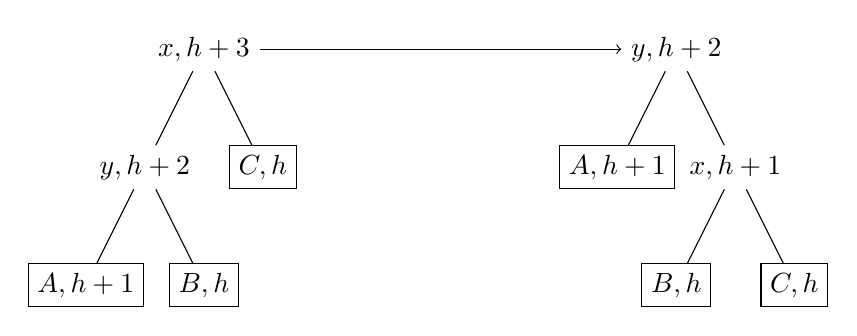
\begin{tikzpicture}
        \node (x1) {$x, h + 3$}
            child {
                node {$y, h + 2$}
                child { node [draw] {$A, h + 1$} }
                child { node [draw] {$B, h$} }
            }
            child {
                node [draw] {$C, h$}
            };
        \node (x2) at (6, 0) {$y, h + 2$}
            child {
                node [draw] {$A, h + 1$}
            }
            child {
                node {$x, h + 1$}
                child { node [draw] {$B, h$} }
                child { node [draw] {$C, h$} }
            };
        \draw[->] (x1) -- (x2);
    \end{tikzpicture}

    \vspace{3em}

    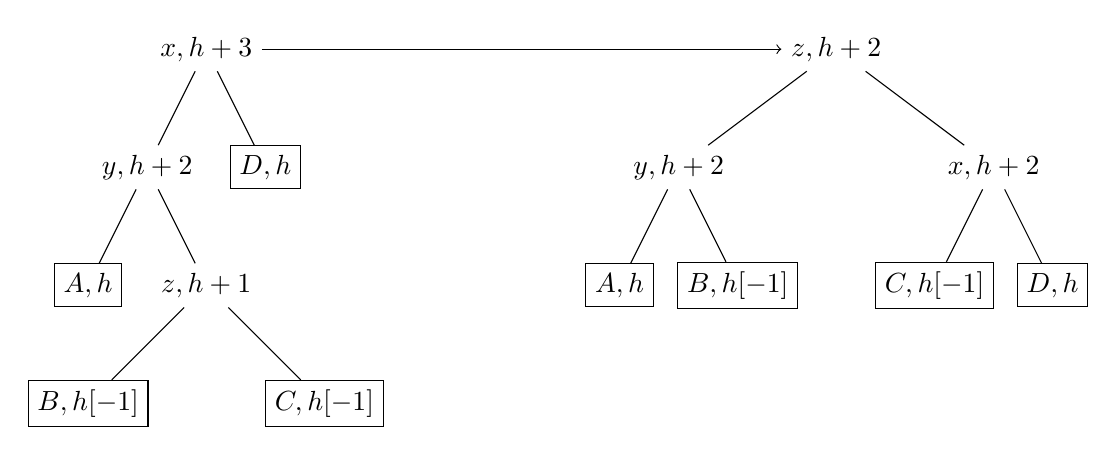
\begin{tikzpicture}
        \node (x1) {$x, h + 3$}
            child {
                node {$y, h + 2$}
                child { node [draw] {$A, h$} }
                child {
                    node {$z, h + 1$}
                    [sibling distance=30mm]
                    child { node [draw] {$B, h [- 1]$} }
                    child { node [draw] {$C, h [- 1]$} }
                }
            }
            child {
                node [draw] {$D, h$}
            };

        \node (x2) at (8, 0) {$z, h + 2$}
            [level 1/.style={sibling distance=40mm}]
            [level 2/.style={sibling distance=15mm}]
            child {
                node {$y, h + 2$}
                child { node [draw] {$A, h$} }
                child { node [draw] {$B, h[-1]$} }
            }
            child {
                node {$x, h + 2$}
                child { node [draw] {$C, h[-1]$} }
                child { node [draw] {$D, h$} }
            };

        \draw[->] (x1) -- (x2);
    \end{tikzpicture}
\end{center}

Докажем, что высота АВЛ-дерева из $n$ вершин --- $\O(\log n)$:
очевидно, при высоте $h$ в дереве не более $2^h - 1$ вершин.
Рассмотрим минимальное количество вершин.
Будем строить АВЛ-дерево, зависящее от высоты, $S(h)$,
следующим образом:

\begin{align*}
    S(0) & = Z \text{ --- null} \\
    S(1) & = \langle Z; Z \rangle \text{ --- лист} \\
    S(h + 2) & = \langle S(h); S(h + 1) \rangle \\
\end{align*}

\begin{statement}
    $S(h)$ --- минимальное АВЛ-дерево высоты $h$.
\end{statement}
\begin{proof}
    Очевидно, $S(0)$ и $S(1)$ минимальны и единственны.

    Пусть доказано, что $S(h)$ и $S(h + 1)$ минимальны.
    АВЛ-дерево высоты $h + 2$ будет иметь два поддерева
    --- высоты $h + 1$ и $h$ или $h + 1$.
    $S(h + 1)$ содержит $S(h)$, поэтому
    $|S(h + 1)| > |S(h)|$, следовательно,
    $S(h)$ --- минимальное возможное поддерево высоты
    $h$ или $h + 1$.

    Тогда
    \begin{align*}
        \forall T \mid h(T) = h + 2 :
        |T| & \ge 1 + \min(|S(h)|; |S(h + 1)|) + |S(h + 1)| = \\
        & = 1 + |S(h)| + |S(h + 1)| = \\
        & = |S(h + 2)| \\
    \end{align*}

    Следовательно, $S(h + 2)$ --- минимальное
    АВЛ-дерево высоты $h + 2$.
\end{proof}

При этом из формулы видно, что
$|S(h + 2)| \ge F(h + 2)$,
и известно, что
\[
    F(n) = \frac{\phi^n - \phi^{-n}}{\sqrt{5}} \in \Theta(\phi^n)
\]

Следовательно,
\begin{gather*}
    \Theta(\phi^n) \le |S(h)| \le 2^h - 1 \\
    h(n) \in \Theta(\log n) \\
\end{gather*}
\qed
